\chapter{Análisis funcional} \label{cap:analisis}

\section{Introducción}

Este capítulo identificará a los tipos de actores que podrán interactuar con el sistema informático que se desea desarrollar. A continuación, se utilizarán los casos de uso y los diagramas de secuencia para describir las acciones que podrán realizar los diferentes actores.

\section{Actores}

Un actor es una representación de una persona, proceso o entidad externa que interactúa con el sistema. Se van a considerar seis tipos de actores:
    \begin{itemize}
        \item Administrador
          \begin{itemize}
              \item Este tipo de usuario estará registrado en el sistema y tendrá un control completo de la aplicación. 
              \item En particular, tendrá las competencias exclusivas de la gestión de todos los tipos de usuarios, centros, juntas, miembros y comisiones. Además, se encargará de la gestión de las copias de seguridad.
          \end{itemize}
          \item Responsable del centro
           \begin{itemize}
               \item Este tipo de usuario estará registrado en el sistema y representará a una persona que podrá gestionar la información de un centro.
               \item En particular, tendrá las competencias exclusivas de la asignación/exclusión a los miembros de gobierno pertenecientes a dicho centro, de creación de las juntas que pertenezcan al centro, así como asignación/exclusión del responsable de cada junta.
            \end{itemize}
            \item Responsable de la junta
           \begin{itemize}
               \item Este tipo de usuario estará registrado en el sistema y representará a una persona que podrá gestionar la información de una junta de centro.
               \item En particular, tendrá las competencias exclusivas de la asignación/exclusión a los miembros de junta pertenecientes a dicha junta, de la gestión de las convocatorias realizadas por la junta, de los miembros que participarán en cada una de las convocatorias de la junta, de creación de las comisiones que pertenezcan a la junta, así como asignación/exclusión del responsable de cada comisión.
            \end{itemize}
          \item Responsable de la comisión 
           \begin{itemize}
               \item Este tipo de usuario estará registrado en el sistema y representará a una persona que podrá gestionar la información de una comisión.
               \item En particular, tendrá las competencias exclusivas de la asignación/exclusión a los miembros pertenecientes a dicha comisión, gestión de las convocatorias realizadas por la comisión, y de los miembros que participarán en cada una de las convocatorias de dicha comisión.
            \end{itemize}
        \item Usuario universitario
            \begin{itemize}
                \item Este tipo de usuario estará registrado en el sistema.
                \item Podrá obtener distintos certificados como pueden ser de situación actual, de centros en los que ha participado como miembro de equipo de gobierno, de juntas a las que ha representado, de comisiones a las que ha pertenecido, de convocatorias en las que ha participado...
              \end{itemize}
        \item Público
        \begin{itemize}
              \item Este tipo de usuario no necesitará estar registrado en el sistema.
              \item Podrá consultar la información pública disponible: comisiones de un centro, miembros actuales de una comisión, consulta de actas aprobadas y pendientes de aprobación,...
          \end{itemize}
     \end{itemize}

\section{Casos de uso}

  Los casos de uso describen las acciones que pueden desarrollar los actores del sistema. Se ha identificado los siguientes casos de uso principales, que son descritos en las secciones que se indican:
    \begin{itemize}
    \item \textbf{CU-0. Diagrama de contexto} (Sección \ref{sec:CU-0}).  
    \item \textbf{CU-1. Consultar información pública} (Sección \ref{sec:CU-1}). 
    \item \textbf{CU-2. Administrar información de usuario} (Sección \ref{sec:CU-2}).
    \item \textbf{CU-3. Administrar comisión} (Sección \ref{sec:CU-3}).
    \item \textbf{CU-4. Administrar junta} (Sección \ref{sec:CU-4}).
    \item \textbf{CU-5. Administrar centro} (Sección \ref{sec:CU-5}).
    \item \textbf{CU-6. Administrar Sistema} (Sección \ref{sec:CU-6}).
\end{itemize}

\subsection{Caso de Uso 0. Diagrama de Contexto}\label{sec:CU-0}         

  El diagrama de contexto engloba los casos de uso principales que componen el sistemas. Véanse la Figura \ref{fig:Diagrama-Contexto} y la Tabla \ref{tab:CU-0}.

%Diagrama de contexto
\begin{figure}[H]
        \centering
        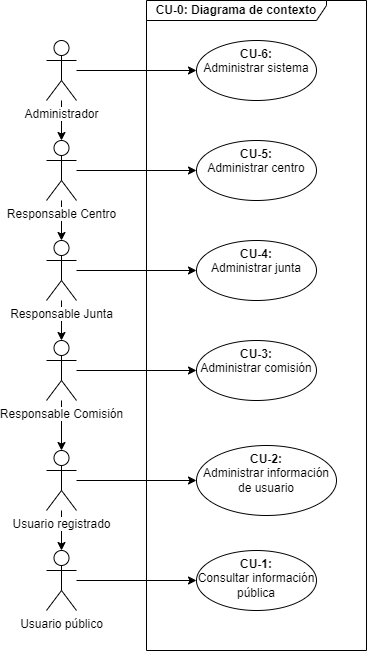
\includegraphics[scale=0.6]{img/diagramas/Funcional/CU-0.png}
        \caption{Diagrama de Contexto}\label{fig:Diagrama-Contexto}
\end{figure}

\begin{table}[H]
\caption{CU-0. Diagrama de contexto}\label{tab:CU-0}
\begin{center}
    \begin{tabular}{|l|p{12cm}|}
    \hline
    \multicolumn{2}{|c|}{Caso de uso 0 - Diagrama de contexto} \\ 
    \hline \hline
    Actores                 &   Público, Usuario registrado, Responsable Comisión,\\ 
                            &  Responsable Junta,  Responsable Centro, Administrador \\ \hline
    Descripción             &   Acciones principales del sistema\\  \hline
    Precondiciones          &   El usuario debe acceder a la página inicial de la aplicación   \\  \hline
    Casos de uso            &   CU-1. Consultar información pública\\  
    & CU-2. Administrar información de usuario\\ 
    & CU-3. Administrar comisión\\
    & CU-4. Administrar junta \\
    & CU-5. Administrar centro \\
    & CU-6. Administrar sistema \\
    \hline
    Flujo principal     &  1a. El usuario público accede a la aplicación sin necesidad de iniciar sesión y podrá consultar la información pública. \\
        & 1b. El resto de usuarios se deberá identificar para acceder a los módulos correspondientes dentro de la aplicación.
    \\ \hline
    Flujo alternativo    & 1. La aplicación no se carga correctamente. \\
      & 2. Se informa del error al usuario. \\
      & 3. Se informa al usuario que puede intentar cargar de nuevo la aplicación.
    \\  \hline
    \end{tabular}
    \end{center}
    \end{table}

\newpage

\subsection{CU-1. Consultar información pública}\label{sec:CU-1}

El caso de uso \textit{CU-1. Consultar información pública} describe las acciones que puede realizar el Usuario Público (véanse la Tabla \ref{tab:CU-1} y la Figura \ref{fig:Diagrama-Caso de uso 1. Consultar información pública}.). Este caso de uso está compuesto por los siguientes sub-casos de uso que se describen en las tablas que se indican:
\begin{itemize}
    \item CU-1.1 Consultar información actual equipos de gobierno(Tabla \ref{tab:CU-1.1}).
    \item CU-1.2 Consultar información actual junta (Tabla \ref{tab:CU-1.2}).
    \item CU-1.3 Consultar información actual comisiones (Tabla \ref{tab:CU-1.3}).
    \item CU-1.4 Consultar información actual convocatorias (Tabla \ref{tab:CU-1.4}).
    \item CU-1.5 Consultar ayuda usuario público (Tabla \ref{tab:CU-1.5}).
\end{itemize}

\begin{figure}[H]
\centering
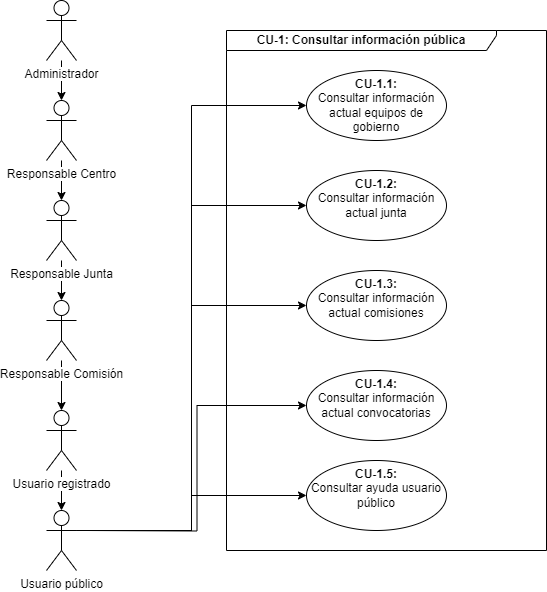
\includegraphics[scale=0.75]{img/diagramas/Funcional/CU-1.png}
\caption{CU-1. Consultar información pública}\label{fig:Diagrama-Caso de uso 1. Consultar información pública}   
\end{figure}

\begin{table}[H]
\caption{CU-1. Consultar información pública}\label{tab:CU-1}
\begin{center}
    \begin{tabular}{|l|p{12cm}|}
    \hline
    \multicolumn{2}{|c|}{Caso de uso 1 - Consultar información pública} \\ 
    \hline \hline
    Actores                 &   Usuario público          \\ \hline
    Descripción             &   Acciones que puede realizar el usuario público \\  \hline
    Precondiciones          &   El usuario debe haber accedido a la página principal de la aplicación y elegido el caso de uso CU-1. Consultar información pública.   \\  \hline
    Casos de uso            &   CU-1.1. Consultar información actual equipos de gobierno \\  
    & CU-1.2. Consultar información actual junta \\ 
    & CU-1.3. Consultar información actual comisiones \\
    & CU-1.4. Consultar información actual convocatorias \\
    & CU-1.5. Consultar ayuda usuario público\\

    \hline
    Flujo principal     &   1. El usuario elige un centro universitario \\ 
    & 2. El sistema muestra la información solicitada en formato organigrama \\ \hline
    Flujo alternativo    &  1. Se produce un error al intentar ejecutar la información elegida. \\ 
                            &  2. Se informa al usuario del error.  \\  
                            &  3. El sistema vuelve a mostrar las opciones disponibles.  \\  \hline    
            \end{tabular}
        \end{center}
    \end{table}

\begin{table}[H]
\caption{CU-1.1 Consultar información actual equipos de gobierno}
        \label{tab:CU-1.1}
        \begin{center}
            \begin{tabular}{|l|p{12cm}|}
                \hline
                \multicolumn{2}{|c|}{Caso de uso 1.1 - Consultar información actual equipos de gobierno} \\ \hline \hline
                Actores                 &   Usuario público          \\  \hline
                Descripción             &   Consultar información pública del equipo de gobierno actual de un centro seleccionado. \\  \hline
                Precondiciones          &   El usuario debe haber accedido a la aplicación y elegido el caso de uso CU-1.1 Consultar información actual equipos de gobierno.  \\  \hline
                Casos de uso            &   \\  \hline
                Flujo principal         &   1. El sistema muestra los centros universitarios   \\
                                        &   2. El usuario escoge un centro universitario    \\ 
                       & 3. El sistema muestra la información pública actual del centro escogido en formato organigrama \\ \hline
                Flujo alternativo    &   1. Se produce un error al intentar mostrar la información de un  centro no universitario. 
                \\  & 2. El sistema informa al usuario de error producido. 
                \\  & 3. El sistema vuelve a mostrar la lista de centros no universitarios.
                \\\hline
            \end{tabular}
        \end{center}
    \end{table}
    
\begin{table}[H]
\caption{CU-1.2 Consultar información actual junta}  \label{tab:CU-1.2}
        \begin{center}
            \begin{tabular}{|l|p{12cm}|}
                \hline
                \multicolumn{2}{|c|}{Caso de uso 1.2 - Consultar información actual junta} \\ \hline \hline
                Actores           &   Usuario público          \\  \hline
                Descripción         &   Consultar información actual junta. \\  \hline
                Precondiciones          &   El usuario debe haber accedido a la aplicación y elegido el caso de uso CU-1.2 Consultar información actual junta  \\  \hline
                Casos de uso            &          \\  \hline
                Flujo principal         &   1. El sistema muestra los centros universitarios.   \\
                &   2. El usuario escoge un centro universitario.    \\                  & 3. El sistema muestra la información pública actual del centro escogido. \\ \hline
                 Flujo alternativo    &   1. Se produce un error al intentar mostrar la información de un  centro  universitario. 
                \\  & 2. El sistema informa al usuario de error producido. 
                \\  & 3. El sistema vuelve a mostrar la lista de centros  universitarios. 
                \\
                \hline
            \end{tabular}
        \end{center}
    \end{table}

\begin{table}[H]
\caption{CU-1.3 Consultar información actual comisiones}  \label{tab:CU-1.3}
        \begin{center}
            \begin{tabular}{|l|p{12cm}|}
                \hline
                \multicolumn{2}{|c|}{Caso de uso 1.3 - Consultar información actual comisiones} \\ \hline \hline
                Actores           &   Usuario público          \\  \hline
                Descripción         &   Consultar información actual comisiones. \\  \hline
                Precondiciones          &   El usuario debe haber accedido a la aplicación y elegido el caso de uso CU-1.3 Consultar información actual comisiones  \\  \hline
                Casos de uso            &          \\  \hline
                Flujo principal         &   1. El sistema muestra los centros universitarios.   \\
                &   2. El usuario escoge un centro universitario.    \\                  & 3. El sistema muestra la información pública actual del centro escogido. \\ \hline
                 Flujo alternativo    &   1. Se produce un error al intentar mostrar la información de un  centro  universitario. 
                \\  & 2. El sistema informa al usuario de error producido. 
                \\  & 3. El sistema vuelve a mostrar la lista de centros  universitarios. 
                \\
                \hline
            \end{tabular}
        \end{center}
    \end{table}

\begin{table}[H]
\caption{CU-1.4 Consultar información actual convocatorias}  \label{tab:CU-1.4}
        \begin{center}
            \begin{tabular}{|l|p{12cm}|}
                \hline
                \multicolumn{2}{|c|}{Caso de uso 1.4 - Consultar información actual convocatorias} \\ \hline \hline
                Actores           &   Usuario público          \\  \hline
                Descripción         &   Consultar información actual convocatorias. \\  \hline
                Precondiciones          &   El usuario debe haber accedido a la aplicación y elegido el caso de uso CU-1.4 Consultar información actual convocatorias  \\  \hline
                Casos de uso            &          \\  \hline
                Flujo principal         &   1. El sistema muestra los centros universitarios.   \\
                &   2. El usuario escoge un centro universitario.    \\                  & 3. El sistema muestra la información pública actual del centro escogido. \\ \hline
                 Flujo alternativo    &   1. Se produce un error al intentar mostrar la información de un  centro  universitario. 
                \\  & 2. El sistema informa al usuario de error producido. 
                \\  & 3. El sistema vuelve a mostrar la lista de centros  universitarios. 
                \\
                \hline
            \end{tabular}
        \end{center}
    \end{table}

\begin{table}[H]
\caption{CU 1.5. Consultar ayuda del usuario público}        \label{tab:CU-1.5}
        \begin{center}
            \begin{tabular}{|l|p{12cm}|}
                \hline
                \multicolumn{2}{|c|}{Caso de uso 1.5 - Consultar ayuda del usuario público} \\ \hline \hline
                Actores                 &   Usuario público \\  \hline
                Descripción             &   Consultar ayuda del usuario público. \\  \hline
                Precondiciones          &  El usuario debe haber accedido a la aplicación y elegido el caso de uso CU-1.5 Consultar ayuda del usuario público. \\  \hline
                Casos de uso            &           \\  \hline
                Flujo principal         &   1. El sistema muestra la información de ayuda al usuario público \\ \hline
                Flujo alternativo    &   1. Se produce un error al intentar mostrar la ayuda al usuario. \\
                & 2. El sistema informa al usuario del error producido. \\
                & 3. El sistema vuelve a mostrar al usuario las opciones disponibles (CU-1. Consultar información pública).  \\
                \hline
            \end{tabular}
        \end{center}
    \end{table}

\newpage

\subsection{CU-2. Administrar información de usuario}\label{sec:CU-2}    

El caso de uso \textit{CU-2. Administrar información de usuario} describe las acciones que puede realizar el Usuario universitario registrado en el sistema (véanse la Tabla \ref{tab:CU-2} y la Figura \ref{fig:Diagrama-Caso de uso 2. Administrar información de usuario}.). Este caso de uso está compuesto por los siguientes sub-casos de uso que se describen en las tablas que se indican:
\begin{itemize}
    \item CU-2.1 Editar información de usuario (Tabla \ref{tab:CU-2.1}).
    \item CU-2.2 Generar certificados (Tabla \ref{tab:CU-2.2}).
    \item CU-2.3 Consultar ayuda (Tabla \ref{tab:CU-2.3}).
\end{itemize}

\begin{figure}[H]
        \centering
        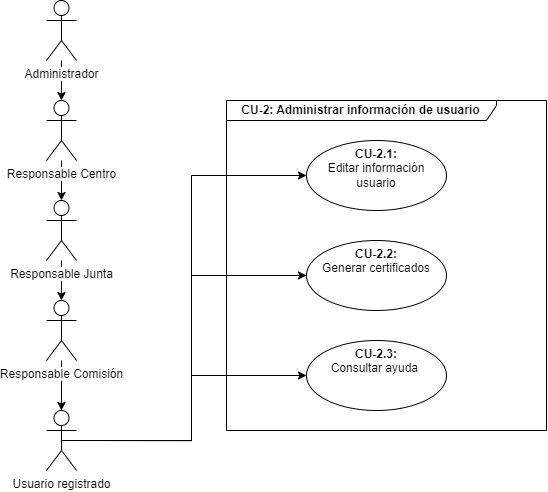
\includegraphics[scale=0.75]{img/diagramas/Funcional/CU-2.png}
        \caption{CU 2. Administrar información de usuario.}
        \label{fig:Diagrama-Caso de uso 2. Administrar información de usuario}
    \end{figure}

\begin{table}[H]
        \caption{CU-2. Administrar información de usuario}
        \label{tab:CU-2}
        \begin{center}
            \begin{tabular}{|l|p{12cm}|}
                \hline
                \multicolumn{2}{|c|}{Caso de uso 2 - Administrar información de usuario} \\ \hline \hline
                Actores                 &   Usuario universitario registrado        \\  \hline
                Descripción             &   Administrar información de usuario. \\  \hline
                Precondiciones          &   El usuario se debe haber identificado como usuario universitario y elegido el caso de uso CU-2 Administrar información de usuario.  \\  \hline
                Casos de uso            &  CU-2.1. Editar información usuario\\ 
                &
                CU-2.2. Generar certificados\\ 
                &
                CU-2.3. Consultar ayuda usuario universitario \\
                \hline
                Flujo principal     &    1. El sistema muestra al usuario universitario las opciones disponibles.\\ 
                &   2. El usuario elige una de las opciones.\\ 
                &   3. El sistema ejecuta la opción elegida por el usuario.\\ 
                \hline
                Flujo alternativo    &  1. Se produce un error al intentar ejecutar la opción elegida. \\ 
                &  2. Se informa al usuario del error.  \\  
                &  3. El sistema vuelve a mostrar las opciones disponibles.  \\
                \hline
            \end{tabular}
        \end{center}
    \end{table}


\begin{table}[H]
    \caption{CU-2.1. Editar información usuario}
    \label{tab:CU-2.1}
    \begin{center}
        \begin{tabular}{|l|p{12cm}|}
            \hline
            \multicolumn{2}{|c|}{Caso de uso 2.1 -Editar información usuario} \\ \hline \hline
            Actores                 &   Usuario universitario registrado          \\  \hline
            Descripción             &   Editar información  del usuario \\  \hline
            Precondiciones          &   El usuario se debe haber identificado como usuario universitario y elegido el caso de uso CU-2.1 Editar información usuario. \\
            \hline
            Casos de uso            &             \\  \hline
            Flujo principal         &   1. El sistema muestra en formato editable la información del usuario   \\
            &   2. El usuario edita la información que proceda.    \\ 
            & 3. El sistema graba los datos actualizados. \\ \hline
            Flujo alternativo    &   1. Se produce un error al editar la información. \\
            & 2. El sistema informa al usuario sobre el error que se ha producido. \\
            & 3. El sistema vuelve a mostrar la opción de editar la información del centro no universitario.
             \\  \hline
        \end{tabular}
    \end{center}
\end{table}

\begin{table}[H]
    \caption{CU-2.2. Generar certificados}
    \label{tab:CU-2.2}
    \begin{center}
        \begin{tabular}{|l|p{12cm}|}
            \hline
            \multicolumn{2}{|c|}{Caso de uso 2.2 -Generar certificados} \\ \hline \hline
            Actores                 &   Usuario universitario registrado          \\  \hline
            Descripción             &   Editar información  del usuario \\  \hline
            Precondiciones          &   El usuario se debe haber identificado como usuario universitario y elegido el caso de uso CU-2.2 Generar certificados. \\
            \hline
            Casos de uso            &             \\  \hline
            Flujo principal         &   1. El sistema muestra una lista de certificados a generar   \\
            &   2. El usuario selecciona el tipo de certificado.    \\ 
            & 3. El sistema genera un PDF con el tipo de certificado seleccionado por el usuario. \\ \hline
            Flujo alternativo    &   1. Se produce un error al seleccionar la información. \\
            & 2. El sistema informa al usuario sobre el error que se ha producido. \\
            & 3. El sistema vuelve a mostrar la opción de selección de la información.
             \\  \hline
        \end{tabular}
    \end{center}
\end{table}


\begin{table}[H]
\caption{CU 2.3. Consultar la ayuda del usuario universitario}        \label{tab:CU-2.3}
        \begin{center}
            \begin{tabular}{|l|p{12cm}|}
                \hline
                \multicolumn{2}{|c|}{Caso de uso 2.3 -  Consultar la ayuda del usuario universitario} \\
                \hline \hline
                Actores                 &   Usuario universitario registrado          \\  
                \hline
                Descripción             &   Consultar la ayuda del usuario universitario. \\  \hline
                Precondiciones          &  El usuario debe haber accedido a la aplicación y elegido el caso de uso CU-2.3 Consultar la ayuda del usuario universitario. \\  
                \hline
                Casos de uso            &           \\  
                \hline
                Flujo principal         &   1. El sistema muestra la información de ayuda al usuario  \\ 
                \hline
                Flujo alternativo    &   1. Se produce un error al intentar mostrar la ayuda del usuario. \\
                & 2. El sistema informa al usuario del error ocurrido. \\
                & 3. El sistema vuelve a mostrar al usuario las opciones disponibles (CU-2. Administrar centro no universitario).  \\
                \hline
            \end{tabular}
        \end{center}
    \end{table}
\newpage


\subsection{CU-3. Administrar comisión}\label{sec:CU-3}    
El caso de uso \textit{CU-3. Administrar comisión} describe las acciones que puede realizar el Usuario responsable de comisión (véanse la Tabla \ref{tab:CU-3} y la Figura \ref{fig:Diagrama-Caso de uso 3. Administrar comisión}). Este caso de uso está compuesto por los siguientes sub-casos de uso que se describen en las tablas que se indican:
\begin{itemize}
  \item CU-3.1 Editar información de comisión responsable (Tabla \ref{tab:CU-3.1}).
  \item CU-3.2 Gestionar miembros de comisión (Tabla \ref{tab:CU-3.2}).
          \begin{itemize}
            \item CU-3.2.1 Buscar miembro de comisión.
            \item CU-3.2.2 Crear  miembro de comisión.
            \item CU-3.2.3 Consultar miembro de comisión.
            \item CU-3.2.4 Modificar miembro de comisión.
            \item CU-3.2.5 Eliminar miembro de comisión.
            \item CU-3.2.6 Asignar/Desasignar responsable miembro de comisión.
        \end{itemize}
  \item CU-3.3 Gestionar convocatorias de comisión (Tabla \ref{tab:CU-3.3}).
          \begin{itemize}
            \item CU-3.3.1 Buscar convocatoria de comisión.
            \item CU-3.3.2 Crear convocatoria de comisión.
            \item CU-3.3.3 Consultar convocatoria de comisión.
            \item CU-3.3.4 Modificar convocatoria de comisión.
            \item CU-3.3.5 Eliminar convocatoria de comisión.
            \item CU-3.3.6 Asignar/Desasignar asistentes convocatoria de comisión.

        \end{itemize}
 \item CU-3.4 Consultar la ayuda del responsable comisión (Tabla \ref{tab:CU-3.4}).
\end{itemize}


\begin{figure}[H]
        \centering
        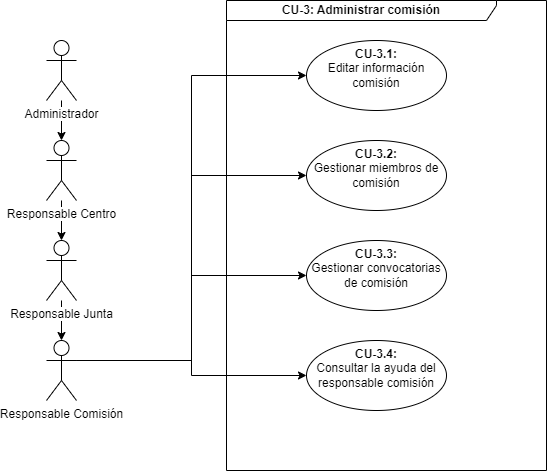
\includegraphics[scale=0.75]{img/diagramas/Funcional/CU-3.png}
        \caption{CU-3. Administrar comisión}
        \label{fig:Diagrama-Caso de uso 3. Administrar comisión}
    \end{figure}
    
\begin{table}[H]
        \caption{CU-3. Administrar comisión}
        \label{tab:CU-3}
        \begin{center}
            \begin{tabular}{|l|p{12cm}|}
                \hline
                \multicolumn{2}{|c|}{Caso de uso 3 - Administrar comisión} \\ \hline \hline
                Actores                 &   Responsable  comisión         \\  \hline
                Descripción             &   Gestión de una comisión. \\  \hline
                Precondiciones          &   El usuario se debe haber identificado como responsable comisión y elegido el caso de uso CU-3. Administrar comisión.  \\  \hline
                Casos de uso            &  CU-3.1. Editar información de comisión responsable. \\ 
                &
                CU-3.2. Gestionar miembros de comisión. \\ 
                &
                CU-3.3. Gestionar convocatorias de comisión. \\ 
                & 
                CU-3.4. Consultar la ayuda del responsable comisión. \\ 
                \hline
                Flujo principal     &    1. El sistema muestra al responsable comisión las opciones disponibles.\\ 
                &   2. El responsable comisión elige una de las opciones.\\ 
                &   3. El sistema ejecuta la opción elegida por el responsable comisión.\\ 
                \hline
                Flujo alternativo    &  1. Se produce un error al intentar ejecutar la opción elegida. \\ 
                &  2. Se informa al usuario del error.  \\  
                &  3. El sistema vuelve a mostrar las opciones disponibles.  \\
                \hline
            \end{tabular}
        \end{center}
    \end{table}

\begin{table}[H]
    \caption{CU-3.1. Editar información de comisión responsable}
    \label{tab:CU-3.1}
    \begin{center}
        \begin{tabular}{|l|p{12cm}|}
            \hline
            \multicolumn{2}{|c|}{Caso de uso 3.1 - Editar información de comisión responsable} \\ \hline \hline
            Actores                 &   Usuario responsable comisión          \\  \hline
            Descripción             &   Editar información  de la comisión. \\  \hline
            Precondiciones          &   El usuario se debe haber identificado como responsable comisión y elegido el caso de uso CU-3.1 Editar información de comisión responsable. \\
            \hline
            Casos de uso            &             \\  \hline
            Flujo principal         &   1. El sistema muestra en formato editable la información de la comisión   \\
            &   2. El responsable comisión edita la información que proceda.    \\ 
            & 3. El sistema graba los datos actualizados. \\ 
            \hline
            Flujo alternativo    &   1. Se produce un error al editar la información. \\
            & 2. El sistema informa al usuario sobre el error que se ha producido. \\
            & 3. El sistema vuelve a mostrar la opción de editar la información de la comisión. \\ 
            \hline
        \end{tabular}
    \end{center}
\end{table}


\begin{table}[H]
    \caption{Gestionar miembros de comisión}
    \label{tab:CU-3.2}
    \begin{center}
        \begin{tabular}{|l|p{12cm}|}
            \hline
            \multicolumn{2}{|c|}{Caso de uso 3.2 - Gestionar miembros de comisión} \\
            \hline \hline
            Actores                 &   Responsable de comisión          \\  
            \hline
            Descripción             &   Permite la gestión de los miembros de la comisión responsable. \\  \hline
            Precondiciones          &   El usuario se debe haber identificado como responsable comisión y elegido el caso de uso CU-3.2 Gestionar miembros de comisión. \\  \hline
            Casos de uso            & 
            3.2.1 Buscar miembro de comisión \\ 
            &
            3.2.2 Crear miembro de comisión \\ 
            & 
            3.2.3. Consultar miembro de comisión\\ 
            & 
            3.2.4 Modificar miembro de comisión \\ 
            &  
            3.2.5 Eliminar miembro de comisión \\ 
            &
            3.2.6 Asignar/Desasignar responsable miembro de comisión \\
            \hline
   
            Flujo principal         &   1. El sistema muestra la lista de los miembros de la comisión responsable.   \\ 
            & 2a. Si no encuentra el miembro de comisión que busca entonces puede crearlo. \\ 
            & 2b. Si encuentra el miembro de comisión que busca entonces puede consultarlo, modificarlo o borrarlo. \\ \hline
            Flujo alternativo    &   1. Se produce un error al intentar ejecutar la opción elegida.  \\ 
            & 2. Se informa del error al usuario. \\
            & 3. El sistema vuelve a mostrar las opciones disponibles. \\
            \hline
        \end{tabular}
    \end{center}
\end{table}

\begin{figure}[H]
        \centering
        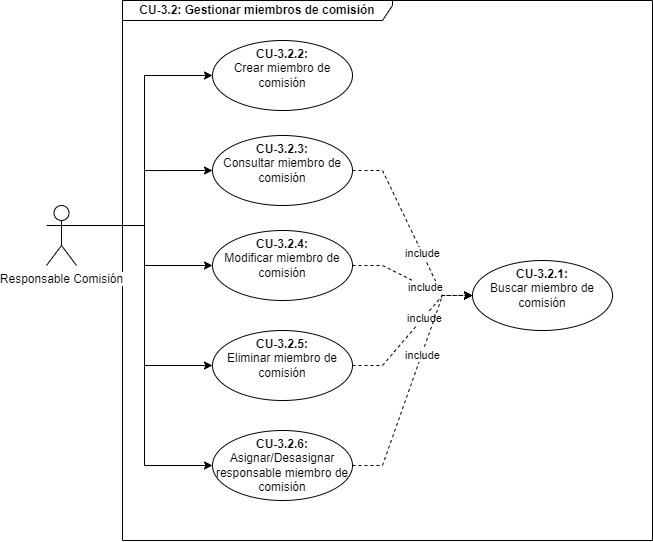
\includegraphics[scale=0.55]{img/diagramas/Funcional/CU-3.2.png}
        \caption{CU-3.2 Gestionar miembros de comisión}
        \label{fig:Diagrama-Caso de uso 3.2 Gestionar miembros de comisión}
    \end{figure}

\begin{table}[H]
    \caption{Gestionar convocatorias de comisión}
    \label{tab:CU-3.3}
    \begin{center}
        \begin{tabular}{|l|p{12cm}|}
            \hline
            \multicolumn{2}{|c|}{Caso de uso 3.3 - Gestionar convocatorias de comisión} \\
            \hline \hline
            Actores                 &   Responsable de comisión          \\  
            \hline
            Descripción             &   Permite la gestión de las convocatorias de la comisión responsable. \\  \hline
            Precondiciones          &   El usuario se debe haber identificado como responsable comisión y elegido el caso de uso CU-3.3 Gestionar convocatorias de comisión. \\  \hline
            Casos de uso            & 
            3.3.1 Buscar convocatoria \\ 
            &
            3.3.2 Crear convocatoria \\ 
            & 
            3.3.3. Consultar convocatoria\\ 
            & 
            3.3.4 Modificar convocatoria \\ 
            &  
            3.3.5 Eliminar convocatoria \\ 
            &
            3.3.6 Asignar/Desasignar asistentes convocatoria de comisión \\
            \hline
   
            Flujo principal         &   1. El sistema muestra la lista de las convocatorias de la comisión responsable.   \\ 
            & 2a. Si no encuentra la convocatoria de comisión que busca entonces puede crearla. \\ 
            & 2b. Si encuentra la convocatoria de comisión que busca entonces puede consultarla, modificarla o borrarla. \\ \hline
            Flujo alternativo    &   1. Se produce un error al intentar ejecutar la opción elegida.  \\ 
            & 2. Se informa del error al usuario. \\
            & 3. El sistema vuelve a mostrar las opciones disponibles. \\
            \hline
        \end{tabular}
    \end{center}
\end{table}

\begin{figure}[H]
        \centering
        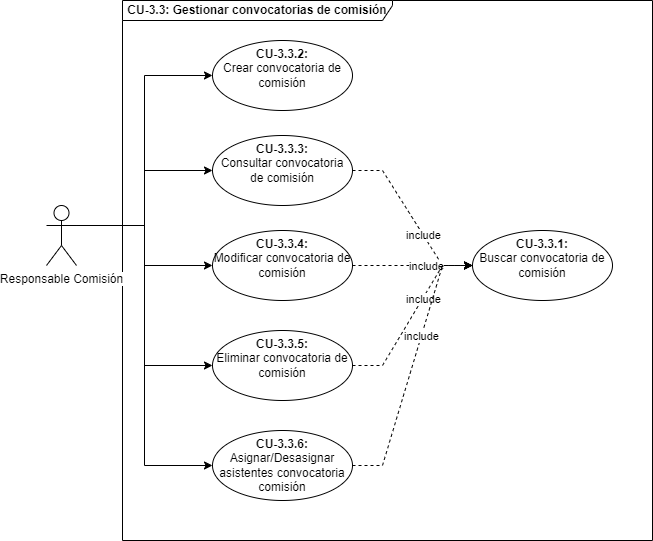
\includegraphics[scale=0.55]{img/diagramas/Funcional/CU-3.3.png}
        \caption{CU-3.3 Gestionar convocatorias de comisión}
        \label{fig:Diagrama-Caso de uso 3.3 Gestionar convocatorias de comisión}
    \end{figure}


\begin{table}[H]
    \caption{Consultar ayuda de responsable comisión}
    \label{tab:CU-3.4}
    \begin{center}
        \begin{tabular}{|l|p{12cm}|}
            \hline
            \multicolumn{2}{|c|}{Caso de uso 3.4 - Consultar ayuda de responsable comisión} \\ \hline 
            Actores                 &   Responsable comisión          \\  
            \hline
            Descripción        & Consultar ayuda de responsable comisión    \\ \hline 
            Precondiciones          &   El usuario debe identificarse  como responsable comisión y seleccionar el caso de uso CU-3.4 Consultar ayuda de responsable comisión         \\  \hline
            Casos de uso            &          \\ \hline
            Flujo principal         &   1. El sistema muestra la información de ayuda 
            al usuario responsable comisión.     \\\hline
            Flujo alternativo    &   1. Se produce un error al intentar mostrar la ayuda del usuario \\ 
            & 2. El sistema informa al usuario del error ocurrido. \\ 
            & 3. El sistema vuelve a mostrar al usuario las opciones disponibles (CU-3. Administrar comisión).\\  \hline
        \end{tabular}
    \end{center}
\end{table}

\newpage


\subsection{CU-4. Administrar junta}\label{sec:CU-4}    
El caso de uso \textit{CU-4. Administrar junta} describe las acciones que puede realizar el Usuario responsable de junta (véanse la Tabla \ref{tab:CU-4} y la Figura \ref{fig:Diagrama-Caso de uso 4. Administrar junta}). Este caso de uso está compuesto por los siguientes sub-casos de uso que se describen en las tablas que se indican:
\begin{itemize}
  \item CU-4.1 Editar información de comisión responsable (Tabla \ref{tab:CU-4.1}).
   \item CU-4.2 Gestionar comisiones (Tabla \ref{tab:CU-4.2}).
          \begin{itemize}
            \item CU-4.2.1 Buscar comisión.
            \item CU-4.2.2 Crear comisión.
            \item CU-4.2.3 Consultar comisión.
            \item CU-4.2.4 Modificar comisión.
            \item CU-4.2.5 Eliminar comisión.
        \end{itemize}
  \item CU-4.3 Gestionar miembros de junta (Tabla \ref{tab:CU-4.3}).
          \begin{itemize}
            \item CU-4.3.1 Buscar miembro de junta.
            \item CU-4.3.2 Crear  miembro de junta.
            \item CU-4.3.3 Consultar miembro de junta.
            \item CU-4.3.4 Modificar miembro de junta.
            \item CU-4.3.5 Eliminar miembro de junta.
            \item CU-4.3.6 Asignar/Desasignar responsable miembro de junta.
        \end{itemize}
    \item CU-4.4 Gestionar convocatorias de junta (Tabla \ref{tab:CU-4.4}).
          \begin{itemize}
            \item CU-4.4.1 Buscar convocatoria de junta.
            \item CU-4.4.2 Crear convocatoria de junta.
            \item CU-4.4.3 Consultar convocatoria de junta.
            \item CU-4.4.4 Modificar convocatoria de junta.
            \item CU-4.4.5 Eliminar convocatoria de junta.
            \item CU-4.4.6 Asignar/Desasignar asistentes convocatoria de junta.
        \end{itemize}
 \item CU-4.5 Consultar la ayuda del responsable junta (Tabla \ref{tab:CU-4.5}).
\end{itemize}


\begin{figure}[H]
        \centering
        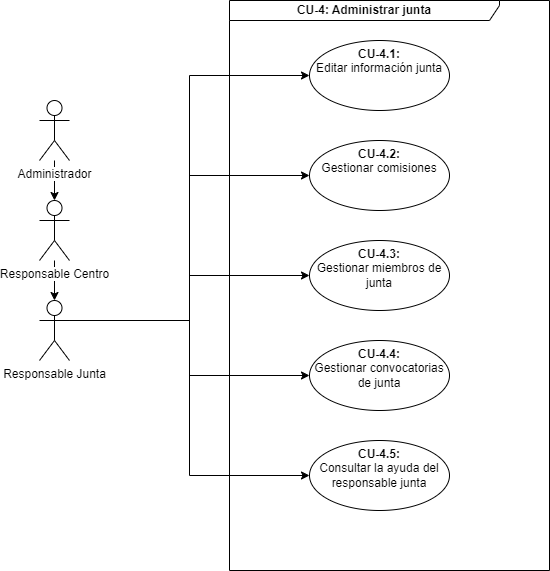
\includegraphics[scale=0.55]{img/diagramas/Funcional/CU-4.png}
        \caption{CU-4. Administrar junta}
        \label{fig:Diagrama-Caso de uso 4. Administrar junta}
    \end{figure}
    
\begin{table}[H]
        \caption{CU-4. Administrar junta}
        \label{tab:CU-4}
        \begin{center}
            \begin{tabular}{|l|p{12cm}|}
                \hline
                \multicolumn{2}{|c|}{Caso de uso 4 - Administrar junta} \\ \hline \hline
                Actores                 &   Responsable junta         \\  \hline
                Descripción             &   Gestión de una junta. \\  \hline
                Precondiciones          &   El usuario se debe haber identificado como responsable junta y elegido el caso de uso CU-4. Administrar junta.  \\  \hline
                Casos de uso            &  CU-4.1. Editar información de junta responsable. \\ 
                &
                CU-4.2. Gestionar comisiones. \\ 
                &
                CU-4.3. Gestionar miembros de junta. \\ 
                &
                CU-4.4. Gestionar convocatorias de junta. \\ 
                & 
                CU-4.5. Consultar la ayuda del responsable junta. \\ 
                \hline
                Flujo principal     &    1. El sistema muestra al responsable junta las opciones disponibles.\\ 
                &   2. El responsable junta elige una de las opciones.\\ 
                &   3. El sistema ejecuta la opción elegida por el responsable junta.\\ 
                \hline
                Flujo alternativo    &  1. Se produce un error al intentar ejecutar la opción elegida. \\ 
                &  2. Se informa al usuario del error.  \\  
                &  3. El sistema vuelve a mostrar las opciones disponibles.  \\
                \hline
            \end{tabular}
        \end{center}
    \end{table}

\begin{table}[H]
    \caption{CU-4.1. Editar información de junta}
    \label{tab:CU-4.1}
    \begin{center}
        \begin{tabular}{|l|p{12cm}|}
            \hline
            \multicolumn{2}{|c|}{Caso de uso 4.1 - Editar información de junta} \\ \hline \hline
            Actores                 &   Usuario responsable junta          \\  \hline
            Descripción             &   Editar información  de la junta. \\  \hline
            Precondiciones          &   El usuario se debe haber identificado como responsable junta y elegido el caso de uso CU-4.1 Editar información de junta responsable. \\
            \hline
            Casos de uso            &             \\  \hline
            Flujo principal         &   1. El sistema muestra en formato editable la información de la junta   \\
            &   2. El responsable junta edita la información que proceda.    \\ 
            & 3. El sistema graba los datos actualizados. \\ 
            \hline
            Flujo alternativo    &   1. Se produce un error al editar la información. \\
            & 2. El sistema informa al usuario sobre el error que se ha producido. \\
            & 3. El sistema vuelve a mostrar la opción de editar la información de la junta. \\ 
            \hline
        \end{tabular}
    \end{center}
\end{table}

\begin{table}[H]
    \caption{Gestionar comisiones}
    \label{tab:CU-4.2}
    \begin{center}
        \begin{tabular}{|l|p{12cm}|}
            \hline
            \multicolumn{2}{|c|}{Caso de uso 4.2 - Gestionar comisiones} \\
            \hline \hline
            Actores                 &   Responsable de junta          \\  
            \hline
            Descripción             &   Permite la gestión de las comisiones de la junta responsable. \\  \hline
            Precondiciones          &   El usuario se debe haber identificado como responsable junta y elegido el caso de uso CU-4.2 Gestionar comisiones de junta. \\  \hline
            Casos de uso            & 
            4.2.1 Buscar comisión \\ 
            &
            4.2.2 Crear comisión \\ 
            & 
            4.2.3. Consultar comisión\\ 
            & 
            4.2.4 Modificar comisión \\ 
            &  
            4.2.5 Eliminar comisión \\ 
            &
            4.2.6 Asignar/Desasignar responsable de comisión \\
            \hline
   
            Flujo principal         &   1. El sistema muestra la lista de las comisiones de la junta responsable.   \\ 
            & 2a. Si no encuentra la comisión que busca entonces puede crearla. \\ 
            & 2b. Si encuentra la comisión que busca entonces puede consultarla, modificarla o borrarla. \\ \hline
            Flujo alternativo    &   1. Se produce un error al intentar ejecutar la opción elegida.  \\ 
            & 2. Se informa del error al usuario. \\
            & 3. El sistema vuelve a mostrar las opciones disponibles. \\
            \hline
        \end{tabular}
    \end{center}
\end{table}

\begin{figure}[H]
        \centering
        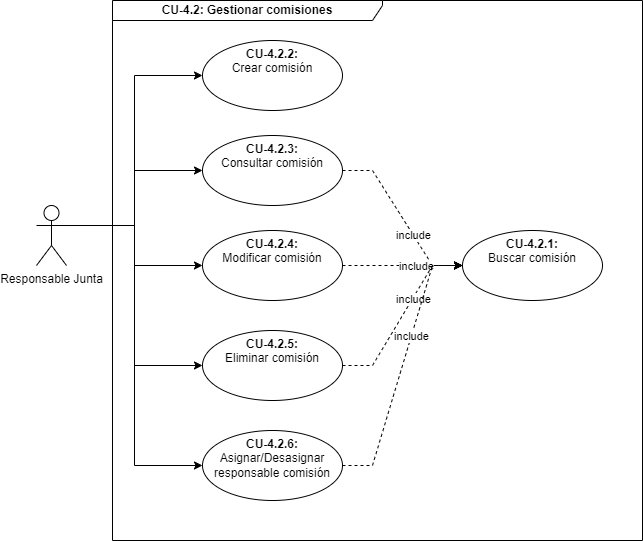
\includegraphics[scale=0.55]{img/diagramas/Funcional/CU-4.2.png}
        \caption{CU-4.2 Gestionar comisiones}
        \label{fig:Diagrama-Caso de uso 4.2 Gestionar comisiones}
    \end{figure}


\begin{table}[H]
    \caption{Gestionar miembros de junta}
    \label{tab:CU-4.3}
    \begin{center}
        \begin{tabular}{|l|p{12cm}|}
            \hline
            \multicolumn{2}{|c|}{Caso de uso 4.3 - Gestionar miembros de junta} \\
            \hline \hline
            Actores                 &   Responsable de junta          \\  
            \hline
            Descripción             &   Permite la gestión de los miembros de la junta responsable. \\  \hline
            Precondiciones          &   El usuario se debe haber identificado como responsable junta y elegido el caso de uso CU-4.3 Gestionar miembros de junta. \\  \hline
            Casos de uso            & 
            4.3.1 Buscar miembro de junta \\ 
            &
            4.3.2 Crear  miembro de junta \\ 
            & 
            4.3.3. Consultar miembro de junta\\ 
            & 
            4.3.4 Modificar miembro de junta \\ 
            &  
            4.3.5 Eliminar miembro de junta \\ 
            &
            4.3.6 Asignar/Desasignar responsable miembro de junta \\
            \hline
   
            Flujo principal         &   1. El sistema muestra la lista de los miembros de la junta responsable.   \\ 
            & 2a. Si no encuentra el miembro de junta que busca entonces puede crearlo. \\ 
            & 2b. Si encuentra el miembro de junta que busca entonces puede consultarlo, modificarlo o borrarlo. \\ \hline
            Flujo alternativo    &   1. Se produce un error al intentar ejecutar la opción elegida.  \\ 
            & 2. Se informa del error al usuario. \\
            & 3. El sistema vuelve a mostrar las opciones disponibles. \\
            \hline
        \end{tabular}
    \end{center}
\end{table}

\begin{figure}[H]
        \centering
        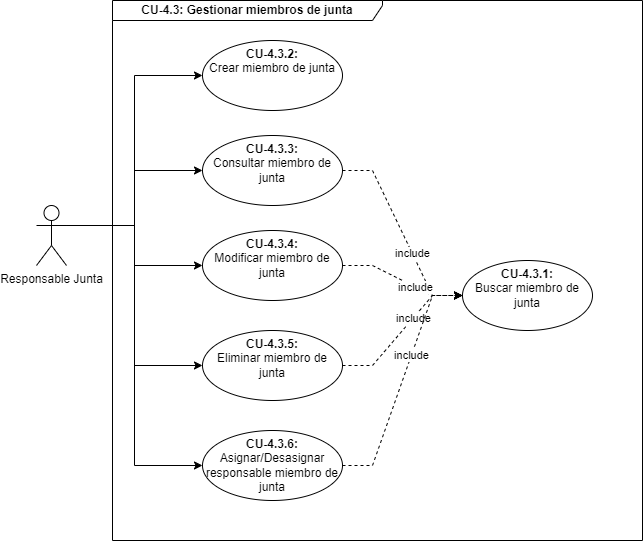
\includegraphics[scale=0.55]{img/diagramas/Funcional/CU-4.3.png}
        \caption{CU-4.3 Gestionar miembros de junta}
        \label{fig:Diagrama-Caso de uso 4.3 Gestionar miembros de junta}
    \end{figure}

\begin{table}[H]
    \caption{Gestionar convocatorias de junta}
    \label{tab:CU-4.4}
    \begin{center}
        \begin{tabular}{|l|p{12cm}|}
            \hline
            \multicolumn{2}{|c|}{Caso de uso 4.4 - Gestionar convocatorias de junta} \\
            \hline \hline
            Actores                 &   Responsable de junta          \\  
            \hline
            Descripción             &   Permite la gestión de las convocatorias de la junta responsable. \\  \hline
            Precondiciones          &   El usuario se debe haber identificado como responsable \textbf{comisión} y elegido el caso de uso CU-4.4 Gestionar convocatorias de junta. \\  \hline
            Casos de uso            & 
            4.4.1 Buscar convocatoria \\ 
            &
            4.4.2 Crear convocatoria \\ 
            & 
            4.4.3. Consultar convocatoria\\ 
            & 
            4.4.4 Modificar convocatoria \\ 
            &  
            4.4.5 Eliminar convocatoria \\ 
            &
            4.4.6 Asignar/Desasignar responsable convocatoria de junta \\
            \hline
   
            Flujo principal         &   1. El sistema muestra la lista de las convocatorias de la junta responsable.   \\ 
            & 2a. Si no encuentra la convocatoria de junta que busca entonces puede crearla. \\ 
            & 2b. Si encuentra la convocatoria de junta que busca entonces puede consultarla, modificarla o borrarla. \\ \hline
            Flujo alternativo    &   1. Se produce un error al intentar ejecutar la opción elegida.  \\ 
            & 2. Se informa del error al usuario. \\
            & 3. El sistema vuelve a mostrar las opciones disponibles. \\
            \hline
        \end{tabular}
    \end{center}
\end{table}

\begin{figure}[H]
        \centering
        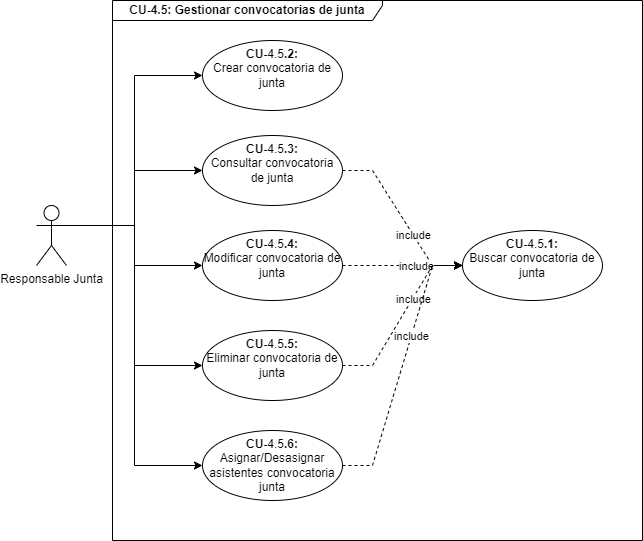
\includegraphics[scale=0.55]{img/diagramas/Funcional/CU-4.4.png}
        \caption{CU-4.4 Gestionar convocatorias de junta}
        \label{fig:Diagrama-Caso de uso 4.4 Gestionar convocatorias de junta}
    \end{figure}


\begin{table}[H]
    \caption{Consultar ayuda de responsable junta}
    \label{tab:CU-4.5}
    \begin{center}
        \begin{tabular}{|l|p{12cm}|}
            \hline
            \multicolumn{2}{|c|}{Caso de uso 4.5 - Consultar ayuda de responsable junta} \\ \hline 
            Actores                 &   Responsable junta          \\  
            \hline
            Descripción        & Consultar ayuda de responsable junta    \\ \hline 
            Precondiciones          &   El usuario debe identificarse  como responsable junta y seleccionar el caso de uso CU-4.5 Consultar ayuda de responsable junta         \\  \hline
            Casos de uso            &          \\ \hline
            Flujo principal         &   1. El sistema muestra la información de ayuda 
            al usuario responsable junta.     \\\hline
            Flujo alternativo    &   1. Se produce un error al intentar mostrar la ayuda del usuario \\ 
            & 2. El sistema informa al usuario del error ocurrido. \\ 
            & 3. El sistema vuelve a mostrar al usuario las opciones disponibles (CU-4. Administrar junta).\\  \hline
        \end{tabular}
    \end{center}
\end{table}

\newpage


\subsection{CU-5. Administrar centro}\label{sec:CU-5}    
El caso de uso \textit{CU-5. Administrar centro} describe las acciones que puede realizar el Usuario responsable de centro (véanse la Tabla \ref{tab:CU-5} y la Figura \ref{fig:Diagrama-Caso de uso 5. Administrar centro}). Este caso de uso está compuesto por los siguientes sub-casos de uso que se describen en las tablas que se indican:
\begin{itemize}
  \item CU-5.1 Editar información de centro responsable (Tabla \ref{tab:CU-5.1}).
  \item CU-5.2 Gestionar juntas (Tabla \ref{tab:CU-5.2}).
          \begin{itemize}
            \item CU-5.2.1 Buscar junta.
            \item CU-5.2.2 Crear junta.
            \item CU-5.2.3 Consultar junta.
            \item CU-5.2.4 Modificar junta.
            \item CU-5.2.5 Eliminar junta.
            \item CU-5.2.6 Asignar/Desasignar responsable de junta 

        \end{itemize}
  \item CU-5.3 Gestionar miembros de gobierno (Tabla \ref{tab:CU-5.3}).
          \begin{itemize}
            \item CU-5.3.1 Buscar miembro de gobierno.
            \item CU-5.3.2 Crear  miembro de gobierno.
            \item CU-5.3.3 Consultar miembro de gobierno.
            \item CU-5.3.4 Modificar miembro de gobierno.
            \item CU-5.3.5 Eliminar miembro de gobierno.
            \item CU-5.3.6 Asignar/Desasignar responsable miembro de gobierno.
        \end{itemize}
  
 \item CU-5.4 Consultar la ayuda del responsable centro (Tabla \ref{tab:CU-5.4}).
\end{itemize}


\begin{figure}[H]
        \centering
        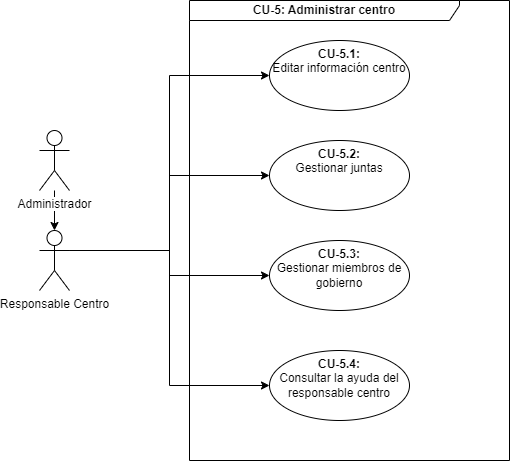
\includegraphics[scale=0.55]{img/diagramas/Funcional/CU-5.png}
        \caption{CU-5. Administrar centro}
        \label{fig:Diagrama-Caso de uso 5. Administrar centro}
    \end{figure}
    
\begin{table}[H]
        \caption{CU-5. Administrar centro}
        \label{tab:CU-5}
        \begin{center}
            \begin{tabular}{|l|p{12cm}|}
                \hline
                \multicolumn{2}{|c|}{Caso de uso 5 - Administrar centro} \\ \hline \hline
                Actores                 &   Responsable centro         \\  \hline
                Descripción             &   Gestión de un centro. \\  \hline
                Precondiciones          &   El usuario se debe haber identificado como responsable centro y elegido el caso de uso CU-5. Administrar centro.  \\  \hline
                Casos de uso            &  CU-5.1. Editar información de centro responsable. \\ 
                &
                CU-5.2. Gestionar juntas. \\ 
                &
                CU-5.3. Gestionar miembros de gobierno. \\ 
                &
                CU-5.4. Consultar la ayuda del responsable centro. \\ 
                \hline
                Flujo principal     &    1. El sistema muestra al responsable centro las opciones disponibles.\\ 
                &   2. El responsable centro elige una de las opciones.\\ 
                &   3. El sistema ejecuta la opción elegida por el responsable centro.\\ 
                \hline
                Flujo alternativo    &  1. Se produce un error al intentar ejecutar la opción elegida. \\ 
                &  2. Se informa al usuario del error.  \\  
                &  3. El sistema vuelve a mostrar las opciones disponibles.  \\
                \hline
            \end{tabular}
        \end{center}
    \end{table}

\begin{table}[H]
    \caption{CU-5.1. Editar información de centro}
    \label{tab:CU-5.1}
    \begin{center}
        \begin{tabular}{|l|p{12cm}|}
            \hline
            \multicolumn{2}{|c|}{Caso de uso 5.1 - Editar información de centro} \\ \hline \hline
            Actores                 &   Usuario responsable centro          \\  \hline
            Descripción             &   Editar información  de la centro. \\  \hline
            Precondiciones          &   El usuario se debe haber identificado como responsable centro y elegido el caso de uso CU-5.1 Editar información de centro responsable. \\
            \hline
            Casos de uso            &             \\  \hline
            Flujo principal         &   1. El sistema muestra en formato editable la información del centro   \\
            &   2. El responsable centro edita la información que proceda.    \\ 
            & 3. El sistema graba los datos actualizados. \\ 
            \hline
            Flujo alternativo    &   1. Se produce un error al editar la información. \\
            & 2. El sistema informa al usuario sobre el error que se ha producido. \\
            & 3. El sistema vuelve a mostrar la opción de editar la información del centro. \\ 
            \hline
        \end{tabular}
    \end{center}
\end{table}

\begin{table}[H]
    \caption{Gestionar juntas}
    \label{tab:CU-5.2}
    \begin{center}
        \begin{tabular}{|l|p{12cm}|}
            \hline
            \multicolumn{2}{|c|}{Caso de uso 5.2 - Gestionar juntas} \\
            \hline \hline
            Actores                 &   Responsable de centro          \\  
            \hline
            Descripción             &   Permite la gestión de las juntas del centro responsable. \\  \hline
            Precondiciones          &   El usuario se debe haber identificado como responsable centro y elegido el caso de uso CU-5.2 Gestionar juntas de centro. \\  \hline
            Casos de uso            & 
            5.2.1 Buscar junta \\ 
            &
            5.2.2 Crear junta \\ 
            & 
            5.2.3. Consultar junta\\ 
            & 
            5.2.4 Modificar junta \\ 
            &  
            5.2.5 Eliminar junta \\ 
            &
            5.2.6 Asignar/Desasignar responsable de junta \\
            \hline
   
            Flujo principal         &   1. El sistema muestra la lista de las juntas del centro responsable.   \\ 
            & 2a. Si no encuentra la junta que busca entonces puede crearla. \\ 
            & 2b. Si encuentra la junta que busca entonces puede consultarla, modificarla o borrarla. \\ \hline
            Flujo alternativo    &   1. Se produce un error al intentar ejecutar la opción elegida.  \\ 
            & 2. Se informa del error al usuario. \\
            & 3. El sistema vuelve a mostrar las opciones disponibles. \\
            \hline
        \end{tabular}
    \end{center}
\end{table}

\begin{figure}[H]
        \centering
        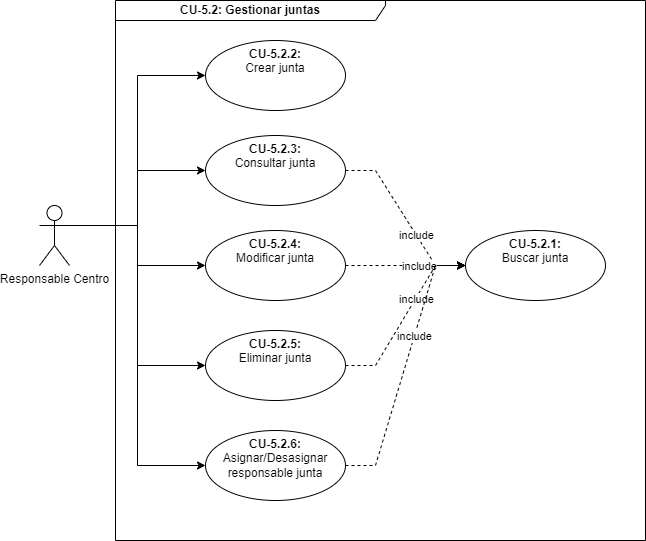
\includegraphics[scale=0.55]{img/diagramas/Funcional/CU-5.2.png}
        \caption{CU-5.2 Gestionar juntas}
        \label{fig:Diagrama-Caso de uso 5.2 Gestionar juntas}
    \end{figure}


\begin{table}[H]
    \caption{Gestionar miembros de gobierno}
    \label{tab:CU-5.3}
    \begin{center}
        \begin{tabular}{|l|p{12cm}|}
            \hline
            \multicolumn{2}{|c|}{Caso de uso 5.3 - Gestionar miembros de gobierno} \\
            \hline \hline
            Actores                 &   Responsable de centro          \\  
            \hline
            Descripción             &   Permite la gestión de los miembros de gobierno del centro responsable. \\  \hline
            Precondiciones          &   El usuario se debe haber identificado como responsable centro y elegido el caso de uso CU-5.3 Gestionar miembros de gobierno. \\  \hline
            Casos de uso            & 
            5.3.1 Buscar miembro de gobierno \\ 
            &
            5.3.2 Crear  miembro de gobierno \\ 
            & 
            5.3.3. Consultar miembro de gobierno\\ 
            & 
            5.3.4 Modificar miembro de gobierno \\ 
            &  
            5.3.5 Eliminar miembro de gobierno \\ 
            &
            5.3.6 Asignar/Desasignar responsable miembro de gobierno \\
            \hline
   
            Flujo principal         &   1. El sistema muestra la lista de los miembros de gobierno del centro responsable.   \\ 
            & 2a. Si no encuentra el miembro de gobierno que busca entonces puede crearlo. \\ 
            & 2b. Si encuentra el miembro de gobierno que busca entonces puede consultarlo, modificarlo o borrarlo. \\ \hline
            Flujo alternativo    &   1. Se produce un error al intentar ejecutar la opción elegida.  \\ 
            & 2. Se informa del error al usuario. \\
            & 3. El sistema vuelve a mostrar las opciones disponibles. \\
            \hline
        \end{tabular}
    \end{center}
\end{table}

\begin{figure}[H]
        \centering
        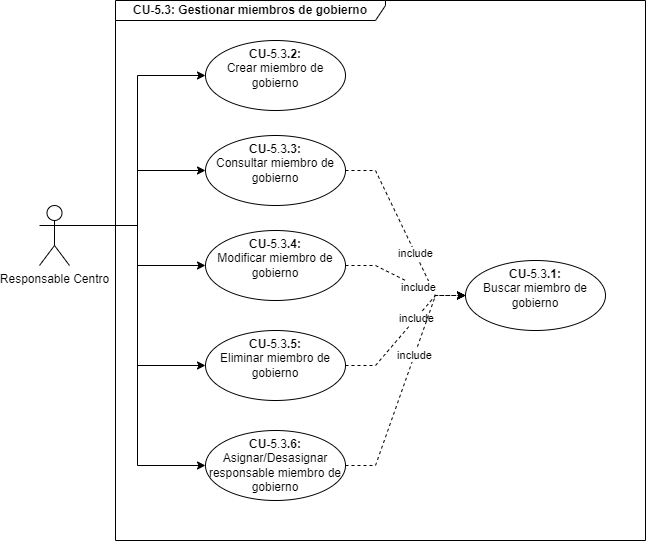
\includegraphics[scale=0.55]{img/diagramas/Funcional/CU-5.3.png}
        \caption{CU-5.3 Gestionar Gestionar miembros de gobierno}
        \label{fig:Diagrama-Caso de uso 5.3 Gestionar miembros de gobierno}
    \end{figure}


\begin{table}[H]
    \caption{Consultar ayuda de responsable centro}
    \label{tab:CU-5.4}
    \begin{center}
        \begin{tabular}{|l|p{12cm}|}
            \hline
            \multicolumn{2}{|c|}{Caso de uso 5.4 - Consultar ayuda de responsable centro} \\ \hline 
            Actores                 &   Responsable centro          \\  
            \hline
            Descripción        & Consultar ayuda de responsable centro    \\ \hline 
            Precondiciones          &   El usuario debe identificarse  como responsable centro y seleccionar el caso de uso CU-5.4 Consultar ayuda de responsable centro         \\  \hline
            Casos de uso            &          \\ \hline
            Flujo principal         &   1. El sistema muestra la información de ayuda 
            al usuario responsable centro.     \\\hline
            Flujo alternativo    &   1. Se produce un error al intentar mostrar la ayuda del usuario \\ 
            & 2. El sistema informa al usuario del error ocurrido. \\ 
            & 3. El sistema vuelve a mostrar al usuario las opciones disponibles (CU-5. Administrar centro).\\  \hline
        \end{tabular}
    \end{center}
\end{table}

\newpage


\subsection{CU-6. Administrar sistema}\label{sec:CU-6}    
El caso de uso \textit{CU-6. Administrar sistema  } describe las acciones que puede realizar el Usuario Administrador (véanse la Tabla \ref{tab:CU-6} y la Figura \ref{fig:Diagrama-Caso de uso 6. Administrar sistema}). Este caso de uso está compuesto por los siguientes sub-casos de uso que se describen en las tablas que se indican:
\begin{itemize}
  \item CU-6.1 Gestionar usuarios (Tabla \ref{tab:CU-6.1}).
  \item CU-6.2 Gestionar centros (Tabla \ref{tab:CU-6.2}).
  \item CU-6.3 Consultar la ayuda del administrador  (Tabla \ref{tab:CU-6.3}).
\end{itemize}

    \begin{table}[H]
        \caption{Administrar sistema}
        \label{tab:CU-6}
        \begin{center}
            \begin{tabular}{|l|p{10cm}|}
                \hline
                \multicolumn{2}{|c|}{Caso de uso 6 - Administrar sistema} \\ \hline \hline
                Actores                 &   Administrador        \\  \hline
                Descripción             &   Gestión del sistema. \\  \hline
                Precondiciones          &   El usuario se debe haber identificado como administrador y elegido el caso de uso CU-6. Administrar sistema           \\  \hline
                Casos de uso            
                & CU-6.1. Gestionar usuarios \\  
                & CU-6.2. Gestionar centros \\ 
                & CU-6.3. Consultar la ayuda del administrador \\
                \hline
                Flujo principal     & 1. El sistema muestra al administrador las opciones disponibles \\ 
                & 2. El administrador elige una de las opciones \\ 
                & 3. El sistema ejecuta la opción elegida. \\ 
                \hline
                Flujo alternativo    &   1. Error al ejecutar la opción elegida, \\ 
                & 2. Se informa al usuario del error ocurrido. \\ 
                & 3. El sistema vuelve a mostrar las opciones disponibles.  \\  
                \hline
            \end{tabular}
        \end{center}
    \end{table}
    
\begin{figure}[H]
        \centering
        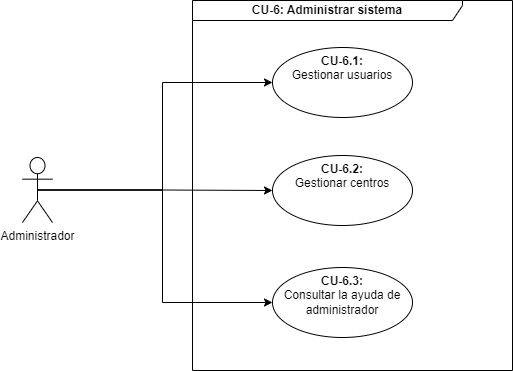
\includegraphics[scale=0.55]{img/diagramas/Funcional/CU-6.png}
        \caption{CU-6. Administrar sistema}
        \label{fig:Diagrama-Caso de uso 6. Administrar sistema}
\end{figure}

\begin{table}[H]
    \caption{Gestionar usuarios}
    \label{tab:CU-6.1}
    \begin{center}
        \begin{tabular}{|l|p{12cm}|}
            \hline
            \multicolumn{2}{|c|}{Caso de uso 6.1 - Gestionar usuarios} \\ \hline \hline

            Actores                 &   Administrador\\  \hline
            Descripción             &   GEstionar información de un usuario universitario. \\  \hline
            Precondiciones          &   El usuario debe ser administrador  y escoger el caso de uso CU-6.1 Gestionar usuarios.        \\  \hline
            Casos de uso            & 6.1.1. Buscar usuario  \\ 
            & 6.1.2. Crear usuario \\ 
            & 6.1.3. Consultar usuario \\ 
            & 6.1.4. Modificar usuario \\ 
            & 6.1.5. Borrar usuario \\    
            \hline
            Flujo principal         &   1. El sistema muestra el listado de usuarios.   \\ 
            & 2a. Si no encuentra el usuario buscado, puede crearlo. \\ 
            & 2b. Si lo encuentra entonces lo puede consultar, modificar o eliminar.  \\ 
            \hline
            Flujo alternativo    &   1. Se produce un error al intentar mostrar la opción  elegida  \\ 
            & 2. El sistema informa al usuario del error. \\ 
            & 3. El sistema vuelve a mostrar al usuario las opciones disponibles.   \\  \hline
            
        \end{tabular}
    \end{center}
\end{table}

\begin{figure}[H]
        \centering
        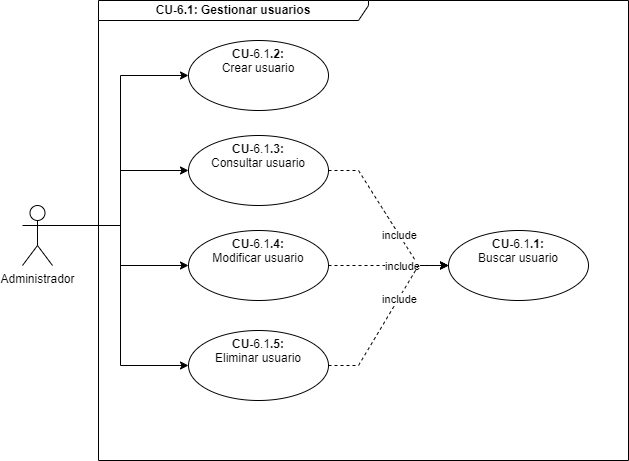
\includegraphics[scale=0.55]{img/diagramas/Funcional/CU-6.1.png}
        \caption{CU-6.1 Gestionar usuarios}
        \label{fig:Diagrama-Caso de uso 6.1 Gestionar usuarios}
\end{figure}


\begin{table}[H]
    \caption{Gestionar centros}
    \label{tab:CU-6.2}
    \begin{center}
        \begin{tabular}{|l|p{12cm}|}
            \hline
            \multicolumn{2}{|c|}{Caso de uso 6.2 - Gestionar centros} \\ \hline \hline
            Actores                 &   Administrador\\  \hline
            Descripción             &   Permite la gestión de los centros universitarios. \\  \hline
            Precondiciones          &   El usuario debe ser administrador y escoger el caso de uso CU-6.2 Gestionar centros.          \\  \hline
            Casos de uso            & 6.2.1. Buscar centro  \\ 
            & 6.2.2. Crear centro \\ 
            & 6.2.3. Consultar centro \\ 
            & 6.2.4. Modificar centro \\ 
            & 6.2.5. Borrar centro \\ 
            \hline
            Flujo principal         &   1. El sistema muestra al administrador las opciones disponibles.   \\ 
            & 2. El administrador elige una de las opciones. \\ 
            & 3. El sistema ejecuta la opción elegida por el administrador. \\ 
            \hline
            Flujo alternativo    &   1. Se produce un error al ejecutar la opción elegida. \\ 
            & 2. Se informa al usuario del error ocurrido. \\ 
            & 3. El sistema vuelve a mostrar las opciones disponibles.  \\  
            \hline
        \end{tabular}
    \end{center}
\end{table}

\begin{figure}[H]
        \centering
        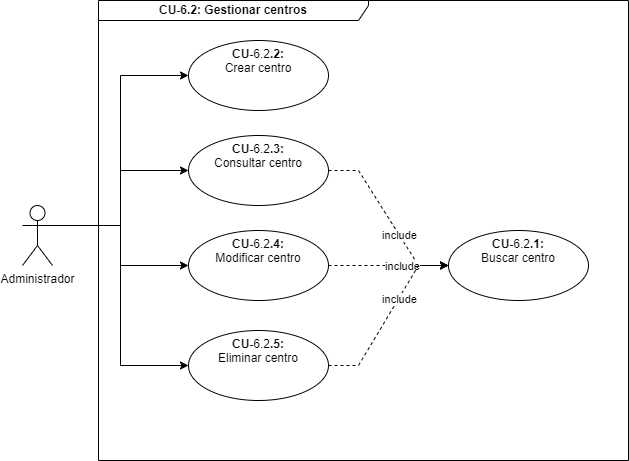
\includegraphics[scale=0.55]{img/diagramas/Funcional/CU-6.2.png}
        \caption{CU-6.2 Gestionar centros}
        \label{fig:Diagrama-Caso de uso 6.2 Gestionar centros}
\end{figure}


\begin{table}[H]
    \caption{Administrar sistema, consultar la ayuda del administrador}
    \label{tab:CU-6.3}
    \begin{center}
        \begin{tabular}{|l|p{12cm}|}
            \hline
            \multicolumn{2}{|c|}{Caso de uso 6.3 - Consultar la ayuda del administrador} \\ \hline \hline

            Actores                 &   Administrador   \\  \hline
            Descripción             &   Permite consultar la ayuda del administrador \\  \hline
            Precondiciones          &   El usuario debe ser administrador y escoger el caso de uso CU-6.3 Consultar la ayuda del administrador.         \\  \hline
            Casos de uso            &   
                                                   \\  \hline
            Flujo principal         &   1. El sistema mostrara la ayuda del administrador.        \\ \hline
            Flujo alternativo    &   1. Se produce un error al intentar mostrar la ayuda del usuario \\ & 2. El sistema informa al usuario del error. \\ & 3. El sistema vuelve a mostrar al usuario las opciones disponibles.   \\  \hline
            
        \end{tabular}
    \end{center}
\end{table}


\newpage

\section{Validación de casos de uso}
La tabla \ref{tab:Validación CU} permite comprobar que los casos de uso cubren todos los requisitos funcionales de la aplicación web propuestos en la Sección \ref{sec:requisitos-funcionales}.
\begin{table}[H]
    \centering
    \caption{Tabla validación casos de uso} \label{tab:Validación CU}
    \begin{tabular}{|l|l|}
        \hline
            \textbf{Requisito funcional} & \textbf{Caso de uso} \\ 
        \hline 
        \hline         
            \textbf{RF-1}  & CU 1.1 \\
            \textbf{RF-2}  & CU 1.2 \\ 
            \textbf{RF-3}  & CU 1.3 \\ 
            \textbf{RF-4}  & CU 1.3 \\ 
            \textbf{RF-5}  & CU 1.4 \\
            \textbf{RF-6}  & CU 1.4 \\ 
            \textbf{RF-7}  & CU 1.5 \\ 
        \hline
            \textbf{RF-8}  & CU 2.1 \\
            \textbf{RF-9}  & CU 2.2 \\
            \textbf{RF-10}  & CU 2.3 \\
        \hline
            \textbf{RF-11}  & CU 3.2 \\
            \textbf{RF-12}  & CU 3.3 \\
            \textbf{RF-13}  & CU 3.4 \\
        \hline
            \textbf{RF-14}  & CU 4.3 \\
            \textbf{RF-15}  & CU 4.2 \\
            \textbf{RF-17}  & CU 4.4 \\
            \textbf{RF-19}  & CU 4.5 \\
        \hline
            \textbf{RF-20}  & CU 5.3 \\
            \textbf{RF-21}  & CU 5.2 \\
            \textbf{RF-27}  & CU 5.4 \\
        \hline
            \textbf{RF-28}  & CU 6.2 \\
            \textbf{RF-36}  & CU 6.3 \\
            \textbf{RF-37}  & CU 6.1 \\

        \hline
    \end{tabular}%
    \end{table}
    
\newpage 

\section{Diagrama de secuencia}

%    El diagrama de secuencia es una representación gráfica que pretende dar una visión de las acciones que se realizarán durante la ejecución de alguna operación en el sistema. A continuación, se muestran los diagramas de secuencias para la creación (Figura  \ref{fig:Diagrama de secuencia crear comisión}), búsqueda (Figura \ref{fig:Diagrama de secuencia consultar comisión}), modificación (Figura \ref{fig:Diagrama de secuencia modificar comisión}) y borrado (Figura \ref{fig:Diagrama de secuencia borrar comisión}) de instancias genéricas (comisiones) que se corresponderán con los tipos de datos que se van a gestionar: centros, juntas, convocatorias, miembros de gobierno, miembros de junta, miembros de comisión, etc.

%\begin{figure}[H]
%        \centering
%        \includegraphics[scale=0.55]{img/diagramas/Secuencia/SEC-1.png}
%        \caption{Diagrama de secuencia de crear comisión}
%        \label{fig:Diagrama de secuencia crear comisión}
%    \end{figure}
    
    
%\begin{figure}[H]
%        \centering
%        \includegraphics[scale=0.55]{img/diagramas/Secuencia/SEC-2.png}
%        \caption{Diagrama de secuencia de consultar comisión}
%        \label{fig:Diagrama de secuencia buscar comisión}
%    \end{figure}
    
%\begin{figure}[H]
%        \centering
%        \includegraphics[scale=0.55]{img/diagramas/Secuencia/SEC-3.png}
%        \caption{Diagrama de secuencia de modificar comisión}
%        \label{fig:Diagrama de secuencia modificar comisión}
%\end{figure}
    
%\begin{figure}[H]
%        \centering
%        \includegraphics[scale=0.55]{img/diagramas/Secuencia/SEC-3.png}
%        \caption{Diagrama de secuencia de borrar comisión}
%        \label{fig:Diagrama de secuencia borrar comisión}
%    \end{figure}


